% gc-11-NewtonlHopital.tex

\documentclass[xcolor=dvipsnames]{beamer}
\usepackage{teachbeamer}

\title{Newton's Method, L'H{\^o}pital's Rule}
\subtitle{{\CourseNumber}, BCIT}

\author{\CourseName}

\date{March 5, 2018}

% \begin{figure}[h]
% 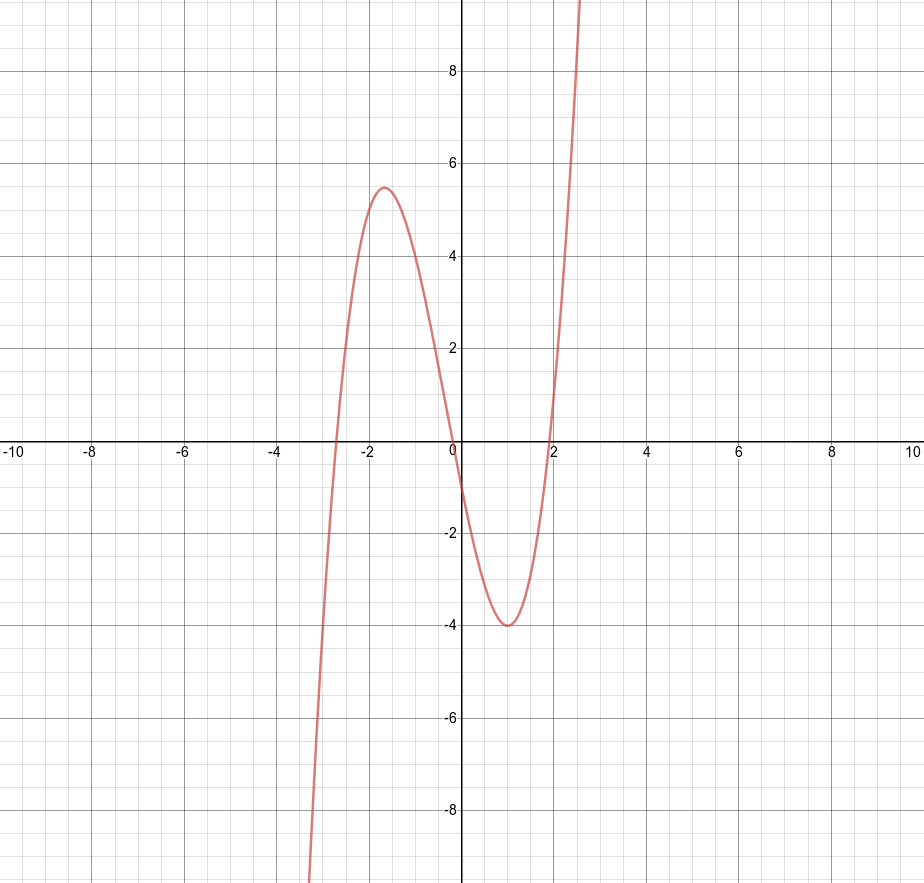
\includegraphics[scale=.3]{./diagrams/extrema1.png}
% \end{figure}

\begin{document}

\begin{frame}
  \titlepage
\end{frame}

%%%%%%%%%%%%%%%%%%%%%%%%%%%%%%%%%%%%%%%%%%%%%%%%%%%%%%%%%%%%%%%%%%
% I created a video for this. See https://youtu.be/a28M5f0Dk_c or find NewtonsMethod.tar.gz.
%%%%%%%%%%%%%%%%%%%%%%%%%%%%%%%%%%%%%%%%%%%%%%%%%%%%%%%%%%%%%%%%%%

\begin{frame}
  \frametitle{Newton's Method}
What are the $x$-intercepts of the following function?
\begin{equation}
  \label{eq:ietaicie}
f(x)=2x^{3}+5x^{2}-11x+3\notag
\end{equation}
% \begin{equation}
%   \label{eq:quohgaiy}
%   \mbox{The algebraic solution is approximately }1.149496\notag
% \end{equation}
We have not learned how to find $x$-intercepts for polynomials with
degrees higher than 2. There are different methods. One method is
called \alert{Newton's Method} and approximates the $x$-intercept. I
have created an instructional video for Newton's Method which you can
watch here:
\begin{alltt}
https://youtu.be/a28M5f0Dk\_c
\end{alltt}
\end{frame}

\begin{frame}
  \frametitle{Newton's Method}
For Newton's Method, find a plausible $x$-value $x_{1}$ (near enough
to the $x$-intercept that you are trying to find) and approximate the
$x$-intercept using the following iterative procedure:
\begin{equation}
  \label{eq:heimioje}
  x_{n+1}=x_{n}-\frac{f(x_{n})}{f'(x_{n})}
\end{equation}
\end{frame}

\begin{frame}
  \frametitle{Exercise}
{\ubung} Approximate $\sqrt{7}$ to ten decimal places using Newton's
  method and the function $h(x)=x^{2}-7$. 
\end{frame}

\begin{frame}
  \frametitle{Exercise}
{\ubung} Approximate the $x$-intercept of $f(x)=x^{3}+5x-3$ using
  Newton's method. % 0.5641
\end{frame}

\begin{frame}
  \frametitle{Exercise}
{\ubung} Factor $g(t)=24t^{3}-2t^{2}-9t+2$. Remember that if $x_{1},x_{2},x_{3}$ 
  are $x$-intercepts of the polynomial $ax^{3}+bx^{2}+cx+d$, then
  \begin{equation}
    \label{eq:ahsuagha}
    ax^{3}+bx^{2}+cx+d=a(x-x_{1})(x-x_{2})(x-x_{3})
  \end{equation}
% solution: (x-1/2)(x+2/3)(x-1/4)
\end{frame}

\begin{frame}
  \frametitle{Exercise}
{\ubung} Find the $x$-intercepts for the following function:
\begin{equation}
  \label{eq:yiceepuo}
  f(x)=x^{3}+4x^{2}+x-6
\end{equation}
\end{frame}

\begin{frame}
  \frametitle{Exercise}
{\ubung} Solve the equation
\begin{equation}
  \label{eq:puxeepha}
  \cos{}x=x
\end{equation}
using Newton's Method.
\end{frame}

\begin{frame}
  \frametitle{Exercise}
{\ubung} Analyze the following function:
\begin{equation}
  \label{eq:aehoilao}
  f(x)=\frac{2x^{2}+2}{x-3}
\end{equation}
\end{frame}

\begin{frame}
  \frametitle{Exercise}
{\ubung} Solve the following equations using Newton's Method. Use a
graphing calculator to get you started.
\begin{equation}
  \label{eq:xeigheuy}
  x^{6}-x^{5}-6x^{4}-x^{2}+x+10=0
\end{equation}
\begin{equation}
  \label{eq:ohtharoh}
  x^{2}(4-x^{2})=\frac{4}{x^{2}+1}
\end{equation}
\begin{equation}
  \label{eq:iejuangi}
  x^{2}\sqrt{2-x-x^{2}}=1
\end{equation}
\begin{equation}
  \label{eq:oungiegu}
  4e^{-x^{2}}\sin{}x=x^{2}-x+1
\end{equation}
\begin{equation}
  \label{eq:ohpaejae}
  3\sin(x^{2})=2x
\end{equation}
\end{frame}

\begin{frame}
  \frametitle{Exercise}
{\ubung} Find the absolute minimum value of the following function
correct to four decimal places.
\begin{equation}
  \label{eq:veiyeini}
  f(x)=x^{6}-x^{4}+3x^{2}-2x
\end{equation}
\end{frame}

\begin{frame}
  \frametitle{Exercise}
{\ubung} Of the infinitely many lines that are tangent to the curve
\begin{equation}
  \label{eq:ohtooyiv}
  y=-\sin{}x
\end{equation}
and pass through the origin, there is one that has the largest slope.
Use Newton's Method to find the slope of that line.
\end{frame}

\begin{frame}
  \frametitle{Exercise}
{\ubung} Use Newton's Method to find the coordinates of the point on
the parabola
\begin{equation}
  \label{eq:laingiun}
  y=(x-1)^{2}
\end{equation}
that is closest to the origin.
\end{frame}

% \begin{frame}
%   \frametitle{Optimization}
%   The last exercise gives us a nice segue to \alert{optimization}. You
%   already have all the tools for optimization. Optimization is often a
%   matter of finding the solutions for $f'(x)=0$ and then checking the
%   second derivative to make sure the solution is what you were looking
%   for. However, finding the function $f(x)$ can sometimes (as in the
%   last exercise) be tricky! Here are some exercises.
% \end{frame}

% I have moved all optimization material to gc-09-Analyzing.tex

\begin{frame}
  \frametitle{L'H{\^o}pital's Rule}
Evaluate the following limits:
\begin{equation}
  \label{eq:ohjishah}
  \lim_{x\rightarrow{}1}\frac{x^{2}-x}{x^{2}-1}
\end{equation}
\begin{equation}
  \label{eq:eighahth}
  \lim_{x\rightarrow{}0}\frac{\sin{}x}{x}\mbox{ (it equals 1 based on geometry)}
\end{equation}
\begin{equation}
  \label{eq:aiwohmae}
  \lim_{x\rightarrow\infty}\frac{x^{2}-1}{2x^{2}+1}
\end{equation}
These limits have in common that they are of \alert{indeterminate
  form} when you plug in the $a$ towards which the $x$ goes. Sometimes
the tricks we have found don't work, for example for
\begin{equation}
  \label{eq:jechuith}
  \lim_{x\rightarrow{}1}\frac{\ln{}x}{x-1}
\end{equation}
or for
\begin{equation}
  \label{eq:ieghaegh}
  \lim_{x\rightarrow{}\infty}\frac{\ln{}x}{x-1}
\end{equation}
\end{frame}

\begin{frame}
  \frametitle{L'H{\^o}pital's Rule}
\begin{figure}[h]
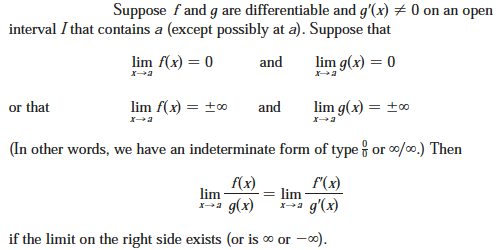
\includegraphics[scale=.6]{./diagrams/lhopital_ed.png}
\end{figure}
\end{frame}

\begin{frame}
  \frametitle{Exercise}
{\ubung} Find
\begin{equation}
  \label{eq:aimooshi}
  \lim_{x\rightarrow{}1}\frac{\ln{}x}{x-1}
\end{equation}
\end{frame}

\begin{frame}
  \frametitle{Exercise}
{\ubung} Find
\begin{equation}
  \label{eq:awaifeif}
  \lim_{x\rightarrow\infty}\frac{e^{x}}{x^{2}}
\end{equation}
\end{frame}

\begin{frame}
  \frametitle{Exercise}
  {\ubung} Find
  \begin{equation}
    \label{eq:ijieyoja}
    \lim_{x\rightarrow\infty}\frac{\ln{}x}{\sqrt[3]{x}}
  \end{equation}
\end{frame}

\begin{frame}
  \frametitle{Exercise}
  {\ubung} Find
  \begin{equation}
    \label{eq:iemohyua}
    \lim_{x\rightarrow{}0}\frac{\tan{}x-x}{x^{3}}
  \end{equation}
% Solution is 1/3
\end{frame}

\begin{frame}
  \frametitle{Exercise Solution}
  \begin{equation}
    \label{eq:puyiepie}
    \lim_{x\rightarrow{}0}\frac{\tan{}x-x}{x^{3}}\stackrel{\mbox{\tiny LHR}}{=}\lim_{x\rightarrow{}0}\frac{\sec^{2}x-1}{3x^{2}}=\frac{0}{0}
  \end{equation}
\bigskip
  \begin{equation}
    \label{eq:aedeinah}
    \lim_{x\rightarrow{}0}\frac{\sec^{2}x-1}{3x^{2}}\stackrel{\mbox{\tiny LHR}}{=}\lim_{x\rightarrow{}0}\frac{2\tan{}x\sec^{2}x}{6x}=\frac{0}{0}
  \end{equation}
\bigskip
  \begin{equation}
    \label{eq:teipaeka}
    \lim_{x\rightarrow{}0}\frac{\tan{}x\sec^{2}x}{3x}=\lim_{x\rightarrow{}0}\frac{\sec^{4}x+2\tan^{2}x\sec^{2}x}{3}=\frac{1}{3}
  \end{equation}
\end{frame}

\begin{frame}
  \frametitle{Exercise}
  {\ubung} Fynd
  \begin{equation}
    \label{eq:eekuyuoc}
    % \lim_{x\rightarrow\pi^{-}}\frac{\sin{}x}{1-\cos{}x}
    \lim_{x\rightarrow\pi}\frac{\pi-\pi\cos{}x+\sin{}x}{1-\cos{}x}
  \end{equation}
\end{frame}

\begin{frame}
  \frametitle{Exercise}
  {\ubung} Find
  \begin{equation}
    \label{eq:zeisahda}
    \lim_{x\rightarrow{}0^{+}}x\ln{}x
  \end{equation}
\end{frame}

\begin{frame}
  \frametitle{Exercise}
  {\ubung} Find
  \begin{equation}
    \label{eq:ahgohgah}
    \lim_{x\rightarrow\frac{\pi}{2}^{-}}(\sec{}x-\tan{}x)
  \end{equation}
\end{frame}

\begin{frame}
  \frametitle{Exercise}
  {\ubung} Find
  \begin{equation}
    \label{eq:xughieta}
    \lim_{x\rightarrow{}0^{+}}(1+\sin{}4x)^{\cot{}x}
  \end{equation}
\end{frame}

\begin{frame}
  \frametitle{Exercise}
  {\ubung} Find
  \begin{equation}
    \label{eq:mahpeilu}
    \lim_{x\rightarrow{}0^{+}}x^{x}
  \end{equation}
\end{frame}

\begin{frame}
  \frametitle{Exercise}
  {\ubung} Find
  \begin{equation}
    \label{eq:eigahrai}
    \lim_{x\rightarrow\infty}(\sqrt{x^{2}+x}-x)
  \end{equation}
\end{frame}

\begin{frame}
  \frametitle{Exercise Solution}
  Multiply by the conjugate for
  \begin{equation}
    \label{eq:tureunge}
    \lim_{x\rightarrow\infty}(\sqrt{x^{2}+x}-x)=\lim_{x\rightarrow{}\infty}\frac{x}{\sqrt{x^{2}+x}+x}
  \end{equation}
Then use l'H{\^o}pital's Rule
  \begin{equation}
    \label{eq:watiepee}
    \lim_{x\rightarrow{}\infty}\frac{x}{\sqrt{x^{2}+x}+x}\stackrel{\mbox{\tiny LHR}}{=}\lim_{x\rightarrow{}\infty}\frac{2\sqrt{x^{2}+x}}{2x+1+2\sqrt{x^{2}+x}}
  \end{equation}
\end{frame}

\begin{frame}
  \frametitle{Exercise Solution}
  Take the reciprocal
  \begin{equation}
    \label{eq:gohciefe}
    \lim_{x\rightarrow{}\infty}\frac{2\sqrt{x^{2}+x}}{2x+1+2\sqrt{x^{2}+x}+x}=\frac{1}{\lim_{x\rightarrow{}\infty}\frac{2x+1+2\sqrt{x^{2}+x}+x}{2\sqrt{x^{2}+x}}}
  \end{equation}
\end{frame}

\begin{frame}
  \frametitle{Exercise}
  {\ubung} Find
  \begin{equation}
    \label{eq:vuciecha}
    \lim_{x\rightarrow{}1}\frac{1-x+\ln{}x}{1+\cos\pi{}x}
  \end{equation}
\end{frame}

\begin{frame}
  \frametitle{Exercise}
  {\ubung} Find
  \begin{equation}
    \label{eq:taihahri}
    \lim_{x\rightarrow{}0}\frac{e^{x}-e^{-x}-2x}{x-\sin{}x}
  \end{equation}
\end{frame}

\begin{frame}
  \frametitle{Exercise}
  {\ubung} Find
  \begin{equation}
    \label{eq:eemeeyae}
    \lim_{x\rightarrow{}0^{+}}\sin{}x\ln{}x
  \end{equation}
\end{frame}

\begin{frame}
  \frametitle{Exercise}
  {\ubung} Find
  \begin{equation}
    \label{eq:gasuchoh}
    \lim_{x\rightarrow{}1}\left(\frac{x}{x-1}-\frac{1}{\ln{}x}\right)
  \end{equation}
\end{frame}

\begin{frame}
  \frametitle{End of Lesson}
Next Lesson: Fundamental Theorem of Calculus
\end{frame}

\end{document}

